%----------------------------------------------------------------------------------------
%	PACKAGES AND OTHER DOCUMENT CONFIGURATIONS
%----------------------------------------------------------------------------------------

\documentclass{article}

\usepackage{fancyhdr} % Required for custom headers
\usepackage{lastpage} % Required to determine the last page for the footer
\usepackage{extramarks} % Required for headers and footers
\usepackage[usenames,dvipsnames]{color} % Required for custom colors
\usepackage{graphicx} % Required to insert images
\usepackage{listings} % Required for insertion of code
\usepackage{caption}
\usepackage{courier} % Required for the courier font
\usepackage{lipsum} % Used for inserting dummy 'Lorem ipsum' text into the template
\usepackage{titlesec}

% My addon
\renewcommand{\thepage}{\Roman{page}}% Roman numerals for page counter
\usepackage{fontspec}   %加這個就可以設定字體
\usepackage{xeCJK}       %讓中英文字體分開設置
\setmainfont{Arial}
\setCJKmainfont{思源黑體} %設定中文為系統上的字型,而英文不去更動,使用原TeX字型
\XeTeXlinebreaklocale "zh"             %這兩行一定要加,中文才能自動換行
\XeTeXlinebreakskip = 0pt plus 1pt     %這兩行一定要加,中文才能自動換行

% \def\footnotesize{\fontsize{16}{24}\selectfont}
\def\small{\fontsize{10}{15}\selectfont}
\def\normalsize{\fontsize{12}{16}\selectfont}
\def\large{\fontsize{16}{24}\selectfont}
\def\Large{\fontsize{20}{30}\selectfont}
\def\LARGE{\fontsize{24}{36}\selectfont}
\def\huge{\fontsize{32}{48}\selectfont}
\def\Huge{\fontsize{36}{54}\selectfont}

% Margins
\topmargin=-0.45in
\evensidemargin=0in
\oddsidemargin=0in
\textwidth=6.5in
\textheight=9.0in
\headsep=0.25in

\linespread{1.1} % Line spacing

% Set up the header and footer
\pagestyle{fancy}
\lhead{\hmwkTitle} % Top left header
% \chead{\hmwkClass\ (\hmwkClassInstructor\ \hmwkClassTime): \hmwkTitle} % Top center head
\rhead{\hmwkClass} % Top right header
% \lfoot{\lastxmark} % Bottom left footer
\cfoot{\thepage} % Bottom center footer
% \rfoot{Page\ \ of\ \protect\pageref{LastPage}} % Bottom right footer
\renewcommand\headrulewidth{0.4pt} % Size of the header rule
% \renewcommand\footrulewidth{0.4pt} % Size of the footer rule

\setlength\parindent{0pt} % Removes all indentation from paragraphs

%----------------------------------------------------------------------------------------
%	CODE INCLUSION CONFIGURATION
%----------------------------------------------------------------------------------------
 
% \definecolor{MyDarkGreen}{rgb}{0.0,0.4,0.0} % This is the color used for comments
% \lstloadlanguages{C++} % Load Perl syntax for listings, for a list of other languages supported see: ftp://ftp.tex.ac.uk/tex-archive/macros/latex/contrib/listings/listings.pdf
% \lstset{language=Matlab, % Use Perl in this example
%         frame=tB, % Single frame around code
%         basicstyle=\normalsize, % Use small true type font
%         % keywordstyle=[1]\color{Blue}\bf, % Perl functions bold and blue
%         % keywordstyle=[2]\color{Purple}, % Perl function arguments purple
%         % keywordstyle=[3]\color{Blue}\underbar, % Custom functions underlined and blue
%         keywordstyle=\color{black}\bfseries\em,
%         keywords={input, output, return, datatype, function, in, if, else, foreach, while, begin, end}, %add the keywords you want, or load a language as Rubens explains in his comment above.
%         identifierstyle=, % Nothing special about identifiers                                         
%         commentstyle=\usefont{T1}{pcr}{m}{sl}\color{MyDarkGreen}\small, % Comments small dark green courier font
%         stringstyle=\color{Purple}, % Strings are purple
%         showstringspaces=false, % Don't put marks in string spaces
%         tabsize=4, % 5 spaces per tab
%         %
%         % Put standard Perl functions not included in the default language here
%         morekeywords={rand},
%         %
%         % Put Perl function parameters here
%         morekeywords=[2]{on, off, interp},
%         %
%         % Put user defined functions here
%         morekeywords=[3]{test},
%        	%
%         morecomment=[l][\color{Blue}]{...}, % Line continuation (...) like blue comment
%         numbers=left, % Line numbers on left
%         firstnumber=1, % Line numbers start with line 1
%         numberstyle=\normalsize, % Line numbers are blue and small
%         stepnumber=1 % Line numbers go in steps of 5
% }

% Creates a new command to include a perl script, the first parameter is the filename of the script (without .pl), the second parameter is the caption
% \newcommand{\algorithmscript}[2]{
% \begin{itemize}
% \item[]\lstinputlisting[caption=#2,label=#1]{#1.NB}
% \end{itemize}
% }

\newcounter{nalg} % defines algorithm counter for chapter-level
\DeclareCaptionLabelFormat{algocaption}{\normalsize\bf Algorithm \thenalg} % defines a new caption label as Algorithm x.y

\lstnewenvironment{algorithm}[1][] %defines the algorithm listing environment
{   
    \refstepcounter{nalg} %increments algorithm number
    \captionsetup{labelformat=algocaption,labelsep=colon} %defines the caption setup for: it ises label format as the declared caption label above and makes label and caption text to be separated by a ':'
    \lstset{ %this is the stype
        frame=tB,
        numbers=left, 
        numberstyle=\normalsize,
        basicstyle=\normalsize, 
        keywordstyle=\color{black}\bfseries\em,
        keywords={,input, output, return, datatype, function, in, if, else, foreach, while, begin, end, } %add the keywords you want, or load a language as Rubens explains in his comment above.
        numbers=left,
        xleftmargin=.04\textwidth,
        #1 % this is to add specific settings to an usage of this environment (for instnce, the caption and referable label)
    }
}
{}

%----------------------------------------------------------------------------------------
%	NAME AND CLASS SECTION
%----------------------------------------------------------------------------------------

\newcommand{\hmwkTitle}{培訓-2} % Assignment title
\newcommand{\hmwkDueDate}{2015年9月23日(火曜日)} % Due date
\newcommand{\hmwkClass}{併查集と狀態空間搜索} % Course/class
\newcommand{\hmwkClassTime}{TTD} % Class/lecture time
\newcommand{\hmwkClassInstructor}{TT} % Teacher/lecturer
\newcommand{\hmwkAuthorName}{FruitTea} % Your name


%----------------------------------------------------------------------------------------
%	TITLE PAGE
%----------------------------------------------------------------------------------------

\title{\hmwkClass}
\author{\hmwkAuthorName}
\date{\hmwkDueDate}

%----------------------------------------------------------------------------------------

\begin{document}
\LARGE~\\[4ex]
\centerline{\bf\hmwkClass}\large\\[2ex]\centerline{\hmwkAuthorName}\\[2ex]\centerline{\hmwkDueDate}\\
\normalsize

\section{Disjoint Sets 互斥集}
\subsection*{Introduction}
Disjoint Sets,又稱互斥集,代表一群集合兩兩交集皆為空集合的狀況,常常用來處理「分類」問題。
因為功能實用、實作簡單,在資訊競賽中很常被使用。\\
實作Disjoint Sets的資料結構我們可以稱她為併查樹(Union-find Tree)或是併查森林(很多棵樹嚴格上來說要叫做森林)。
基本上我們會以一顆併查樹代表一個集合。\\
一個基本的併查樹我們必須實作兩種操作,Find 和 Union。

\subsection{Find 查詢}
我們有一個陣列 P[x] 代表 x 的 parent 是誰,如果 x 是併查樹的樹根(root),我們就把 x 的 parent 當作是自己,
也就是說,一開始所有的 P[x] = x 。(一開始大家都屬於各自不同的集合)\\
如果我們想要知道 x 在哪個集合中(x 的 root 是誰),我們只要遞迴 P[x] 就可以得到答案了。

\begin{algorithm}[caption={Find}, label={alg1}]
function Find(x)
    if x ≠ p[x] then
        return Find(p[x])
    else
        return x
    end if
end function
\end{algorithm}

可是這樣每次找一個點,最慘的狀況下可能會花 O(N) 的時間,所以我們引入一個稱為"Path Compression"的概念,
速度可以快非常多。\\
Path Compression 其實就是在遞迴的過程中,讓所有路徑上的點「直接」連到root。代碼如下。

\begin{algorithm}[caption={Find \& Path Compression}, label={alg1}]
function Find(x)
    if x ≠ p[x] then
        p[x] ← Find(p[x])
        return Find(p[x])
    else
        return x
    end if
end function
\end{algorithm}

\subsection{Union 合併}
想要合併兩個集合,也就是合併兩顆併查樹,只要把A樹的樹根接到B樹的樹根就可以了。

\begin{algorithm}[caption={Union}, label={alg1}]
function Union(x, y)
    p[Find(x)] ← Find(y)
end function
\end{algorithm}

合併上也有一個優化的方法叫做"Union By Rank",也就是把小樹合併到大樹上,這樣需要更動的點會比較少。\\

\subsection{總結}
併查樹可以讓我們在處理分類和合併的問題時可以很輕鬆的完成。如果我們同時使用"Union By Rank"和"Path Compression",
併查樹的複雜度是 O(N × α(N)),其中 α(N) 是阿克曼函數的反函數。不過就算不用"Union By Rank",
複雜度也只是退化到 O(N × lg N),在競賽領域中的操作下,遇到的 α(N) 和 lg N 都不會太大,
所以基本上我們可以把併查樹的複雜度當作 O(N) 來使用。
("Union By Rank"對於併查樹來說會麻煩很多又不會快很多,所以平常大可以不用實作)

\subsection{Exercises!!}

\begin{description}
\item[ 1.]<TIOJ 1312 家族>\\
給你很多組數字 a, b,代表 a 與 b 在同個家族。
現在給你一個數字 k,求 k 所在的家族中編號最小的是誰?
\item[ 2.]<POJ 2492 雌蟲雄蟲>\\
給你很多對關係 x, y,代表蟲 x 跟蟲 y 性別不一樣。
請輸出這些條件是否有任何矛盾 (也就是有蟲為雌雄同體,ex:(x, y)、(y, z)、(z, x))。
\item[ 3.]<POJ 1182 食物鏈>\\
總共有 A、B、C 三種天使,A 吃 B,B 吃 C,C 吃 A。
依序給你很多組關係 d, x, y,若 d = 1 則代表天使 x 跟 y 是同類,d = 2 則代
表天使 x 吃 y。
若當前給的關係與之前的關係矛盾,代表此組關係是假的。
求總共有多少組關係是假的?
\item[ 4.]<TIOJ 1833 陽炎眩亂>\\
有一群蘿莉機器人,分成很多部隊,每個部隊都有一個女王。
題目可能要求你合併兩個部隊或是查詢某隻蘿莉機器人隸屬於哪個女王。
\end{description} 


\section{Search 搜尋}
\subsection*{Introduction}
搜索,也就是暴力的找答案。無論是在空間中還是不同狀態中搜索,總是要試過每個可能性。\\
不過雖然很暴力,但是寫法好或不好差別還是很大的喔!

\subsection{Enumeration 枚舉}
嘗試所有的可能,然後一一檢查,找出答案。

\subsection{State Space Search 狀態空間搜索}
先把問題轉成某種狀態,比如你要去學校上學,一開始在位置(0, 0) 要到位置(s, t)。\\
現在的位置即為狀態。從(0, 0) 到 (0, 1) 就稱為狀態轉移,
比如南海路也許就是一條可以讓你從家裡轉移到學校的其中一個狀態轉移的路徑。\\
所有的狀態的集合就是狀態空間,在這裡面找答案就是所謂的狀態空間搜索。\\
我們並不知道這個稱之為狀態空間的迷宮長怎麼樣,所以我們必須嘗試走走看,至於怎麼走才有效率,
我們介紹幾個常見的演算法。

\subsection{DFS}
Depth First Search(深度優先搜索),簡稱DFS。也就是一直往前走,
直到遇到死路就往後退到上一個岔路並且換一條走,如果所有岔路都走完了就再往後退,直到把所有的點都搜完。
跟著下圖的編號順序走訪一遍就是一個DFS順序的搜尋,當然大家的順序可能不太一樣。\\
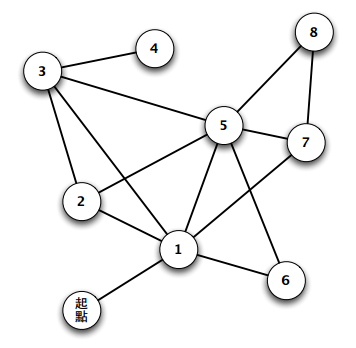
\includegraphics[width=0.5\columnwidth]{DFS.png}\\
實作上,我們只要用遞迴就可以輕鬆完成,也可以用Stack模擬,可是很麻煩。並且注意一定要記的紀錄走過的點。
\begin{algorithm}[caption={DFS}, label={alg1}]
function DFS(v)
    mark v as visited
    for all u that is adjacent to v do
        if u is not visited then
            DFS(u)
        end if
    end for
end function
\end{algorithm}

\subsection{BFS}
Breadth First Search(廣度優先搜索),簡稱BFS,也就是所謂的地毯式搜索。
一層一層的向外擴大搜尋範圍,就像下圖的順序,直到走完所有點。
當然你不可能一次走到很多點,所以下圖的數字代表層數,至於同一層的順序大家可能會不太一樣。
有一個很棒的性質是,BFS的層數剛好就是起點到該點的距離。\\
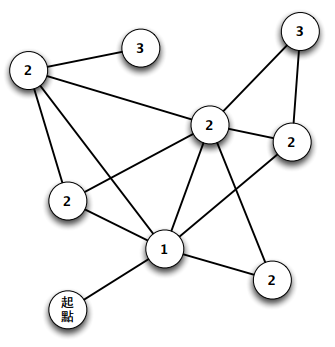
\includegraphics[width=0.5\columnwidth]{BFS.png}\\
實作BFS也很簡單,只要把DFS的Stack換成Queue就可以了。
\begin{algorithm}[caption={BFS}, label={alg1}]
function BFS(v)
    enqueue v to Q (Q is a queue)
    mark v as visited
    while Q is not empty do
        c ← pop Q
        for all u that is adjacent to c do
            if u is not visited then
                push u to Q
                mark u as visited
            end if
        end for
    end while
end function
\end{algorithm}

\subsection{BiBFS}
雙向的BFS,通常是在知道起點和終點而要找最短路徑時,可以交錯從起點和終點做BFS,起點一層,終點一層。
當一個點同時被起點和終點搜到時,我們可以確定一定有一條最短路徑路徑經,從起點過這個點到終點。\\
BiBFS的好處是,一般BFS必須不斷把點存進記憶體裡,假設每個點都連到N個點,那距離 d 的BFS就必須存入O($N^d$)個點。
但是,用BiBFS我們兩個BFS的距離都剩下 $d \over 2$,所以只要存 O($N^{d \over 2}$)個點,省下了不少記憶體。

\subsection{IDDFS}
IDDFS就是限制深度的DFS,先做一個限制深度的DFS,然後不斷加深深度。
這樣做的原因是避免我們走進一個又深又長的死路,白白浪費時間。
因為限制了深度,到達終點時,深度剛好可以代表距離。\\
也許你會覺得這樣一直重複走走過的點很浪費時間,但是從時間複雜度去分析,
假設每個點連到N個點,1~d層點數總共有O($N^{d+1}$),而d+1層卻也有O($N^{d+1}$)個點,所以總共只差了常數時間而已。\\
於是IDDFS就是一個不會浪費空間的BFS,但是比BFS難寫,不過時間複雜度不變。

\subsection{A*}
A*就是把BFS裡的queue換成priority_queue,也就是依照優先度去搜尋,而不是順序。
至於優先度是甚麼呢,其實可以自己定義。A*的優先度是距離終點的估計距離,也就是我們希望靠近終點的優先搜尋。\\
我們給每一點一個優先度 f(x) = g(x) + h(x),其中g(x)代表起點到該點的實際距離,h(x)代表該點到終點的估計距離。
我們只要挑f(x)最小的人先走,很快就可以找到最短路徑。\\
不過這樣真的會是最短路徑嗎?我們可以證明,因為我們不會高估h(x),也就是我們只要保證該點到終點的實際距離 ≥ h(x),
這樣的話如果我們走到終點,其他 f(x)比這條路徑大的路徑都 ≥ 實際距離,這樣這條路徑就是最短路徑了。

\subsection{IDA*}
IDA*就是IDDFS加上A*,也就是限制f(x)的長度。
當我們做IDDFS時,深度(也就是A*裡的g(x))超過限制就砍掉。
現在我們改成f(x)超過長度限制就砍掉(也就是不用g(x)超過限制,如果估計長度超過就可以先砍掉了。)\\
因為我們保證 實際長度 ≥ h(x),所以我們才不會不小心砍掉可以的路徑。

% \subsection{Exercises!!}
% \begin{description}
% \item[ 1.]<Uva 514 Rails>
% \item[ 2.]<TIOJ 1176 Cows>
% \item[ 3.]<TIOJ 1063 最大矩形>
% \item[ 4.]<TIOJ 1489 核心字串>
% \item[ 5.]<HOJ 2 我要寫毛啊>
% \item[ 6.]<TIOJ 1637 我愛台灣>
% \item[ 7.]<TIOJ 1834 炉心融解>
% \end{description}


% \section{雜湊}
% 雜湊、Hash、哈希,是將一群值對應到另外一群值的一種方法。
% 當我們想要從N個元素中尋找某個值的時候,我雖然可以用O(lg N)的時間查找(離散化),
% 但是我們其實並不需要他的位置等等資訊,我們只要確認這個值「存在」與否。
% 理論上Hash可以做到O(1),比如老師點名只需要直接喊你的座號,而不需要從一號開始確認。
% 使用規則對應稱為Hash Function,使用表格對應稱為哈希表。

% \subsection{Hash Function}
% 最簡單的Hash Function就是不要Hash,直接把f(x) = x,優點是絕對不會碰撞,
% 缺點是當數字(或是其他形別資料)範圍太大時很不實用。
% 另外可以透過取餘數(Mod)來建立Hash,又或是其他的對應方法,但是這時我們就必須處理碰撞問題了。

% \subsection{碰撞}
% 因為Hash後的數字範圍較小,所以一定有兩個以上不同的值映射到同一個Hash值,我們稱為碰撞。
% 處理碰撞有幾種作法。
% \begin{description}
% \item[ 1.]RP\\
% 你的人品很好,所以他不會碰撞。
% \item[ 2.]Chaining\\
% 有碰撞就接在同一格後面,但是當碰撞很嚴重時效率會接近沒有Hash。
% \item[ 3.]Linear Probing\\
% 建構新的Hash Function $h(x, i) = (h(x) + i)\ \%\ L$,i從0遞增,直到沒有碰撞為止。當然也可以改成二次多項式$h(x, i) = (h(x) + c_1 i^2 + c_2 i)\ \%\ L$。
% \item[ 4.]Doubly Hashing\\
% 把Hash Function換成這樣:$ h(x, i) = (h_1 (x) + i × h_2 (x))\ mod\ Lׇ$,也就是多Hash幾遍減少碰撞的意思。

% \item[ 5.]Perfect Hashing\\
% 完美雜湊。簡單來說就是先用可能會碰撞的Hash Function先把元素盡量分散,
% 之後再針對每個碰撞的點做絕對不會碰撞的Hash,因為第一層已經讓數量平均分散,所以第二層不會太大。
% \end{description}

% \subsection{Exercises!!}
% \begin{description}
% \item[ 1.]<TIOJ 1160 動態眾數問題>
% \item[ 2.]<TIOJ 1302 撿鞋運動>
% \item[ 3.]<TIOJ 1849 超文字妹妹控協定>
% \end{description}

% \section{STL}
% Standard Template Library,簡稱STL,是一個C++的標準模板庫,提供很多方便的功能可以使用,
% 讓我們可以節省很多編寫資料結構的時間,專注在解題上。
% 他們大多支援類似的method,只要熟悉STL的幾個資料結構,其他的資料結構使用上來說差異不大,
% 只是使用前一定要清楚了解該操作的複雜度和性質(是否有排序等等),否則可能會拖垮效率或甚至出錯。以下筆者大致將常用STL分成了幾項:

% \subsection{資料型態}
% \subsubsection{string}
% C++的string是個很方便的資料型態,讓原本被當成指標的字串可以當成變數傳遞,
% 在編寫函數或是操作字串時更方便,但是在效率上就稍微比C string(字元陣列)慢了。

% \subsection{容器}
% 基本的容器結構,其他STL結構常常使用這些結構當作容器。
% \subsubsection{vector}
% 向量,或是稱做動態陣列,可以自由增加長度。從後端插入均攤O(1)。很常用的容器。
% \subsubsection{list}
% 實做link-list的容器,可以O(1)插入,串接,O(N)查找。
% \subsubsection{deque}
% 較為複雜的容器,雖然功能上是deque(雙頭queue),但是卻可以O(1)隨機查找、O(1)從前後插入刪除。

% \subsection{資料結構}
% \subsubsection{stack}
% 實作stack,預設容器是std::vector,因為std::stack使用一般陣列或是vector取代更為方便,所以不常使用。
% \subsubsection{queue}
% 實作queue,預設容器是std::list,因為實作比較麻煩所以比std::stack較常被使用
% \subsubsection{priority\_queue}
% 實作Heap,預設容器是std::vector,可以O(1)查詢最大值,O(lg N)插入。
% \subsubsection{set/map}
% 實作紅黑樹,set是集合,map是一組key-value對應,基本上可以O(lg N)插入O(lg N)查找
% \subsubsection{unordered set/map}
% 實作Hash,操作跟set/map一樣,但是 unordered set/map 使用Hash,所以可以做到均攤O(1)的效率,
% 如果不需要 set/map 的排序性質建議使用 unordered set/map 。不過因為 unordered set/map 的常數很大,
% 所以在競賽中遇到的情況下通常不會和 set/map 差太多。

% \subsection{STL Algorithm}
% STL模板庫也提供了很多方便的函數,這裡列舉一些常見的函數。
% \subsubsection{sort()/stable\_sort()}
% 排序一個可以遍歷的容器,基本上一般陣列或是vector都可以,如果要穩定排序可以使用stable\_sort()。
% \subsubsection{lower\_bound()、upper\_bound() binary\_search()}
% 分別對一個序列搜尋小於目標的最後一個值、等於目標的最後一個值,和確認目標是否存在該序列中。
% \subsubsection{fill()}
% 將一個序列以某個值填滿,可以用來取代for迴圈設定初始值。
% 和<cstring>中的memset不同的是,memset只能將記憶體規0或是其他有限的操作,
% 但是fill可以填入任何值甚至是物件。
% \subsubsection{random\_shuffle()}
% 隨機排列一個序列,時間複雜度O(N)。
% \subsubsection{reverse()}
% 反轉一個序列。
% \subsubsection{mismatch()}
% 找出兩個序列中第一組不同的值。
% \subsubsection{next\_permutation()}
% 找出下一個排列,\{1,2,3\} -> \{2,1,3\} -> \{2,3,1\}...,當需要每舉排列進行運算時可以使用。


\end{document}